\chapter{前言}
\renewcommand{\baselinestretch}{10.0} %設定行距
\pagenumbering{arabic} %設定頁號阿拉伯數字
\setcounter{page}{1}  %設定頁數
\fontsize{14pt}{2.5pt}\sectionef

%-------------------研究動機與背景------------------------------%
\section{研究動機}
材料分析軟體的應用在機械領域愈來越廣泛,能夠將繪製零件進行分析,但卻鮮少人知道材料分析是怎麼進行的,背後所引用的代碼、原理等。\\
本專題研究方向將由四足機器人作為載體,目的將有限元素分析的公式套入其中計算,進行有限元素分析,利用偏微分方程解出受力情況,才能對零件進行挖空處理,達到輕量化的目的,透過此過程從了解到運動模擬和有限元素法分析等。\\

\begin{figure}[hbt!]
\center
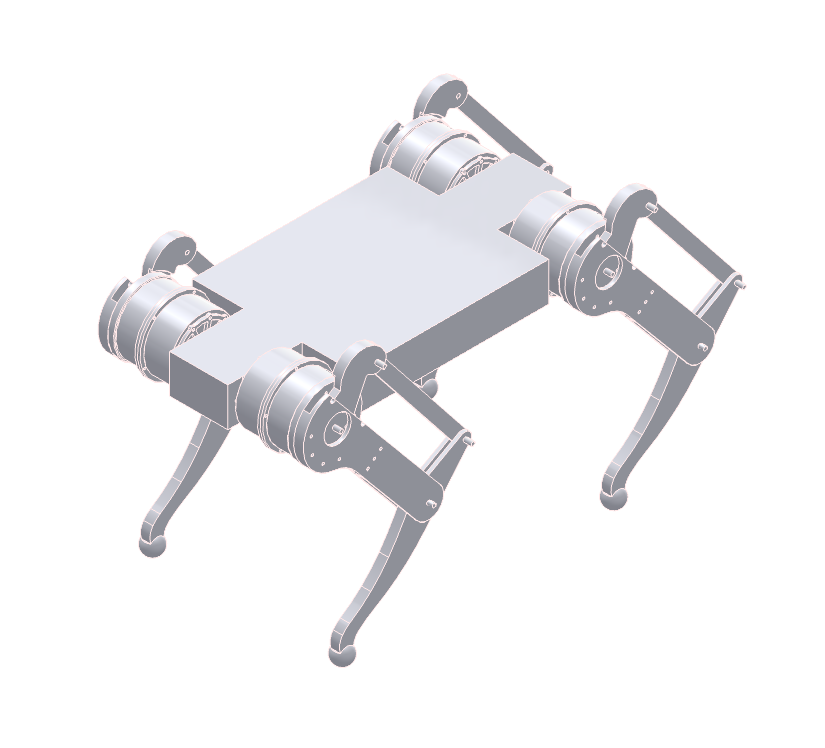
\includegraphics[width=14cm]{四足機器狗}
\caption{\Large 虛擬四足機器人}\label{四足機器狗}
\end{figure}
\newpage
%-----------------------研究目的--------------------------%
\section{研究目的及方法}
\begin{figure}[hbt!]
\begin{center}
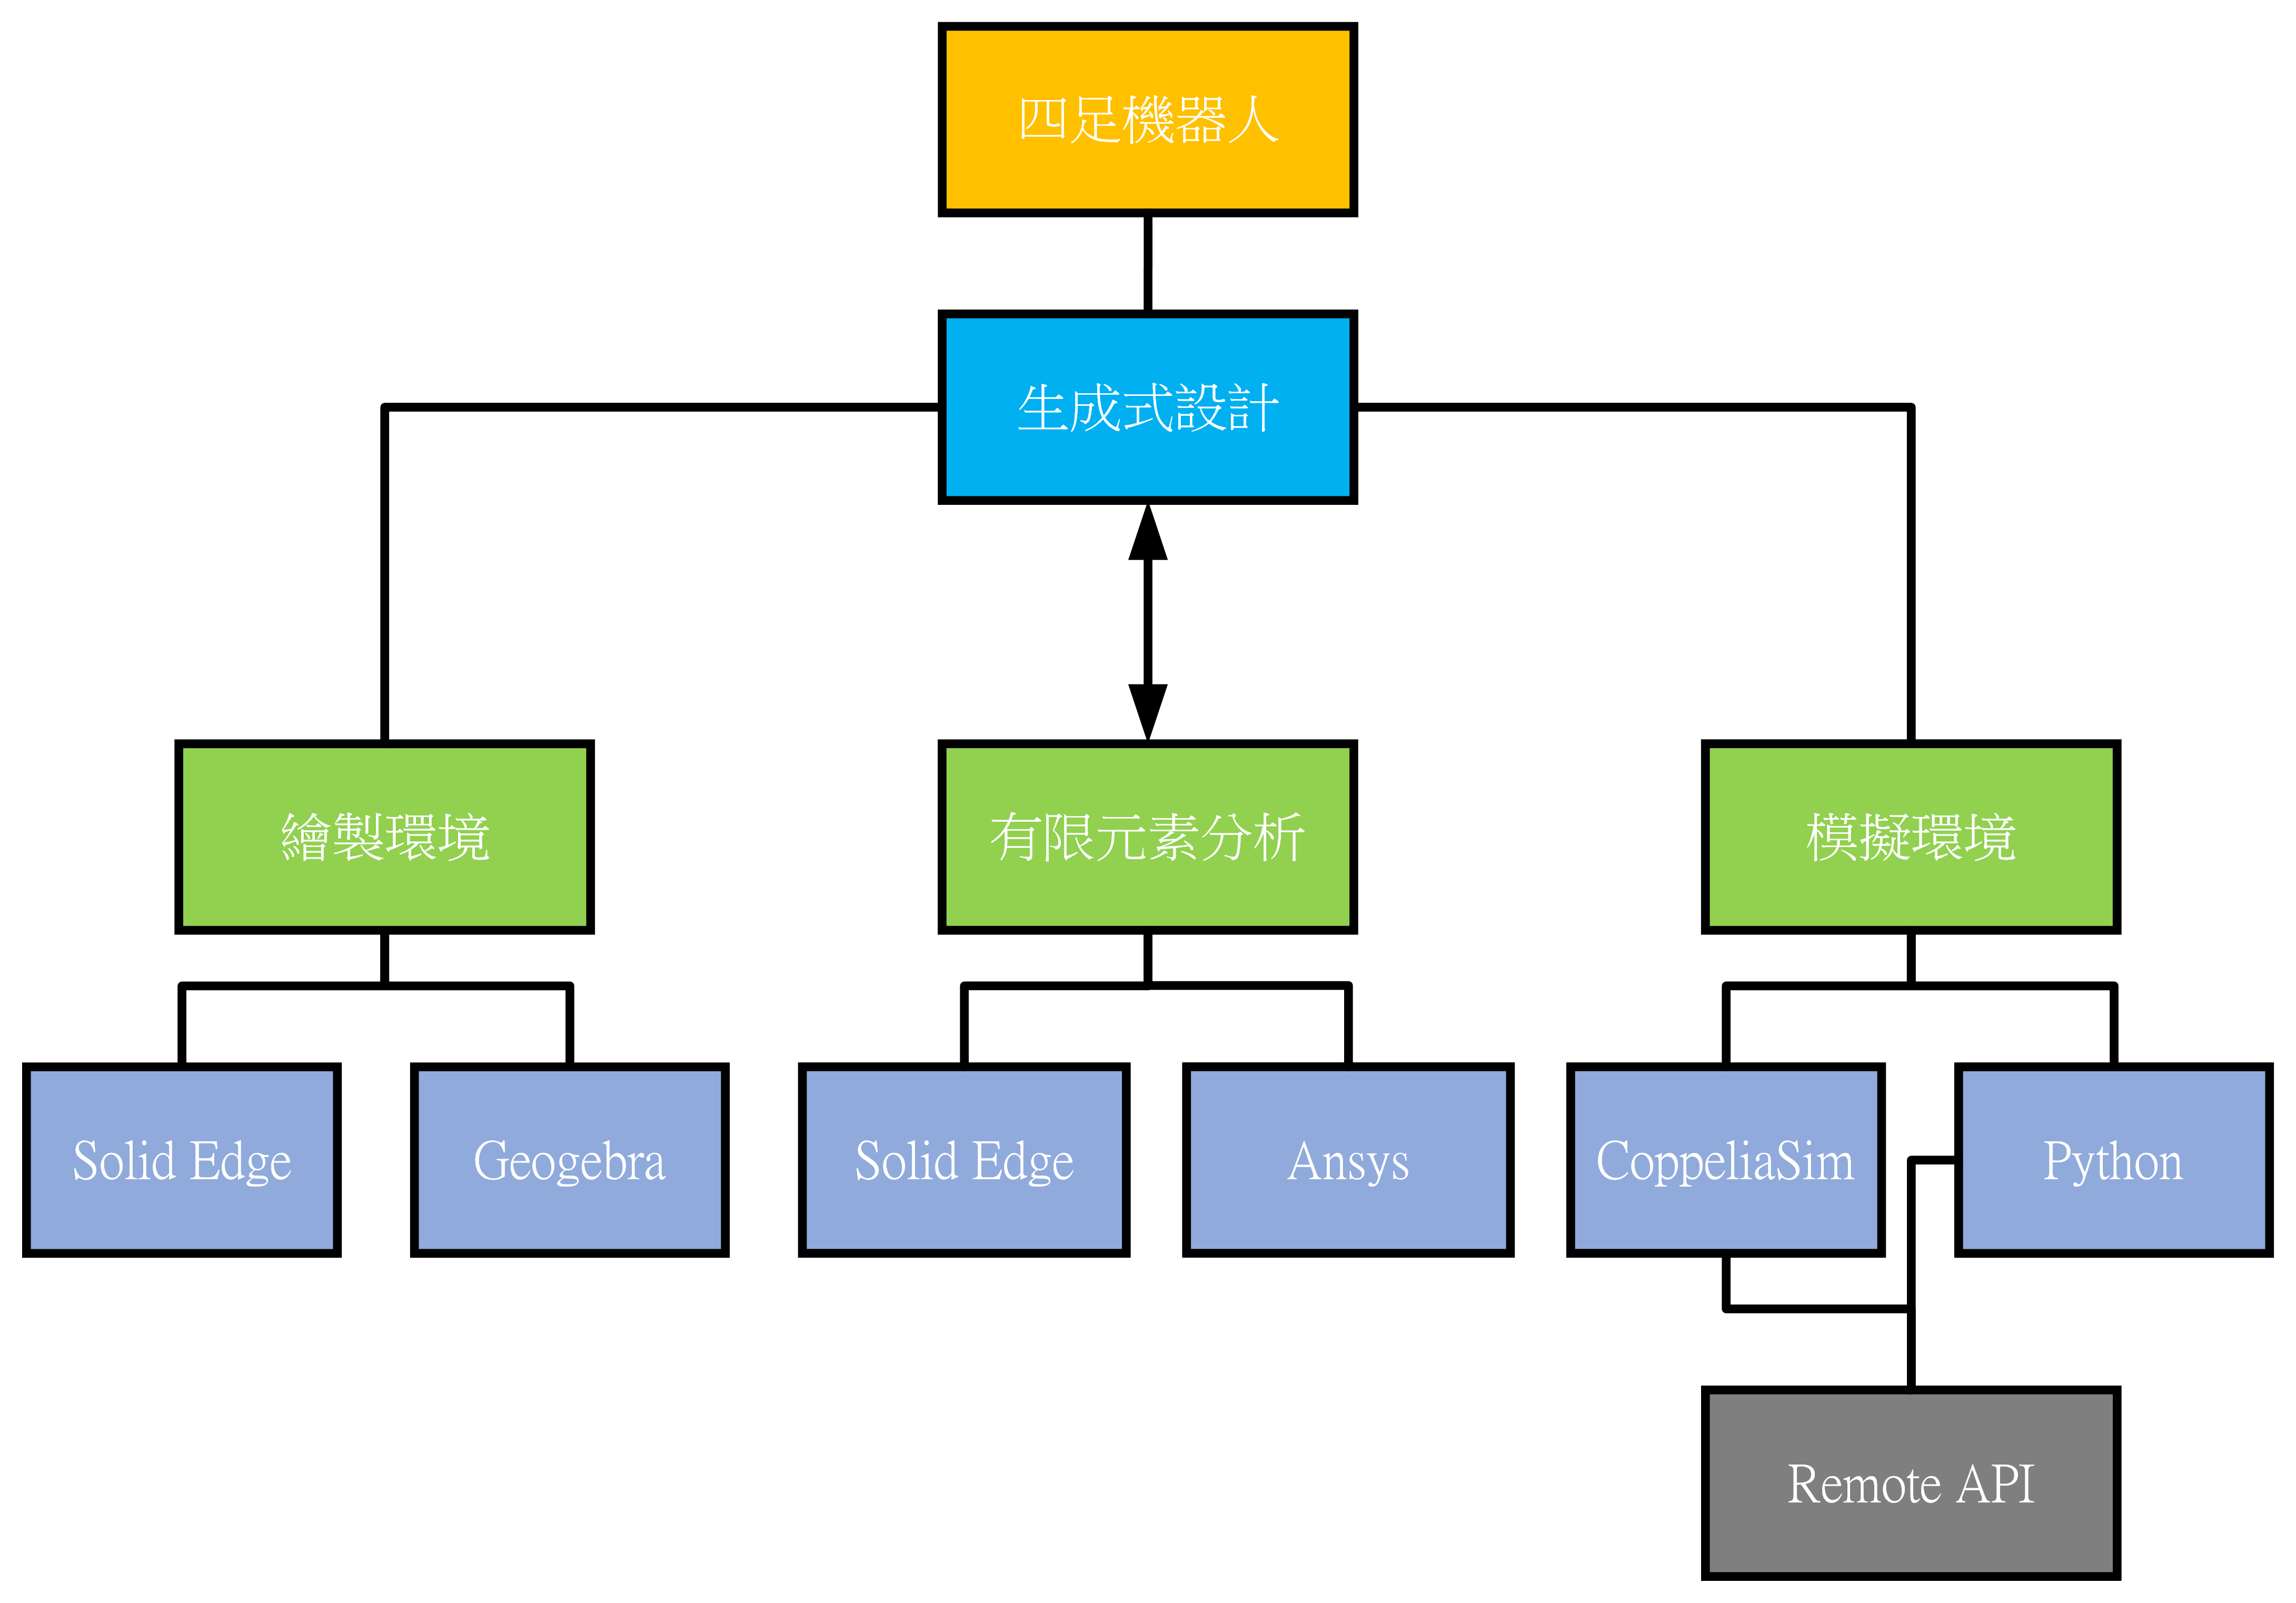
\includegraphics[width=14cm]{研究架構}
\caption{\Large 研究架構}\label{研究架構}
\end{center}
\end{figure}
本專題研究分為三大部分,其一繪製模型,並進行路徑模擬,計算運動軌跡並調整設計,其二將模型導入虛擬環境進行運動模擬,找出運動姿態,其三為利用有限分析法對於零件進行生成式設計,對零件進行優化。\\
參考的四足機器人模型,將其利用Solid Edge繪製並利用GeoGebra進行路徑分析,找出運動軌跡並用此調整連桿參數及推導運動學公式。\\
建立CoppeliaSim模擬環境,導入3D圖檔並組立進行結合,透過Python語言控制各步行機構作動及旋轉角度,以求得各零件最大受力情況,並結合Remote API對四足機器人進行遠端控制。\\
進行有限元素分析,透過上述過程即可得出受力狀況及3D模型,利用Solid Edge即Ansys分析即可得知零件受力狀況(應力、應變、安全係數等),並分別對比兩個軟體分析差異,探討差異原因由何而來,將可對其進行生成式設計,對零件非必要部分做挖空處理,減輕零件重量。\\

%----------------------分析說明------------------------%
\section{專題說明}
此專題主要研究有限元素法在四足機器人上的應用。\\
模型部分參考了資料[1]及Goegebra路徑模擬,繪製出硬體架構,將其視為剛體帶入CoppeliaSim,由於剛體只有一個時間變量,因此可直接計算出物體的受力方向,不受撓曲影響。\\
將受力情況求出後對零件做有限元素分析,此狀態下的零件為柔性狀態,會因為受力不同有變形情況,會產生許多變量,像是位移、速度、加速度等,所以要使用偏微分方程對零件計算,進行離散化、代數方程導入、求解等步驟,此種方法即稱為有限元素法。\\
對比兩軟體分析結果後得出應力、應變等參數後套入到生成式設計,讓電腦進行疊代計算將零件可挖空部分顯示出來,設計者則可以依照需求取捨,對四足機器人步行機構進行挖空處理,節省驅動時所損耗力並同時保有相當程度的堅韌程度。\\

%----------------------文獻探討------------------------%
\section{文獻探討}

\renewcommand{\baselinestretch}{0.5} %設定行距
